\documentclass[10pt]{article}
\usepackage[letterpaper,margin=0.9in]{geometry}
\usepackage[T1]{fontenc}
\usepackage{newtxtext}
\usepackage{microtype}
\usepackage{graphicx}
\usepackage{booktabs}
\usepackage{tabularx}
\usepackage{caption}
\usepackage{enumitem}
\usepackage[hidelinks]{hyperref}
\captionsetup{font=small,labelfont=bf,skip=4pt}
\setlist{nosep,leftmargin=1.3em}
\setlength{\parskip}{3pt}
\setlength{\parindent}{0pt}
\newcommand{\code}[1]{\texttt{\small #1}}
% Team members.
\newcommand{\authors}{Ho-Yen Wu, Jui-Yen Wang, Meng-Chi Tsai}

\title{\vspace{-1.5em}Failure Propagation in a Multi-Agent LLM Workflow:\\
Phase 1 Fault Injection and Measurement in ALFWorld}
\author{\authors\\\small CSE 291A, Fall 2026, Option 5 \quad Code: commit \code{43050fa}}
\date{}

\begin{document}
\maketitle
\vspace{-2.5em}

\section{Introduction}
Our project asks whether tracking the dependencies between agent results can support
efficient recovery while still preserving correct and safe task execution. In Phase~1 we
built a multi-agent LLM baseline on ALFWorld, injected controlled faults into its
intermediate results, and measured how those faults propagate through agent reasoning,
shared memory and the environment. We also measured the two baselines that selective
recovery will have to beat in Phase~2, full restart and always-verify. This report covers
2,360 fault-injection episodes on unseen evaluation games.

Our main observation is that the two kinds of faults behave quite differently. Only 6\% of
accidental faults and 1 of the 306 adversarial faults were masked. Accidental faults changed
the executed actions in 34\% of runs but changed task success in only 0.7\%, so their main
cost is wasted work. Prompt injections changed actions in 77\% of runs and led to
unauthorized actions in 163 of 306 episodes and irreversible actions in 24. We also found that
LLM agents can both filter and amplify faults: corrupted raw observations were absorbed most
often, whereas faults in shared memory could take up to 25 steps to affect an action.

For recovery, full restart costs 1.4--2.9$\times$ a clean episode. Always-verify blocked
every unauthorized action, but it lost more tasks than applying no recovery at all, because
it can detect a fault but has no way of repairing it. Only 61\% of structurally dependent
agent calls actually changed after a fault, and 47\% of faults changed the world state, so we
plan to combine influence-aware recomputation with world-state restoration in Phase~2.

We also characterized failure diversity. The faults produced 92 distinct behavior signatures.
In a 96-episode pilot, a signature-guided fuzzer was about even with random injection on
overall diversity (37 vs.\ 36) but found more severe behaviors (11 vs.\ 8 severe signatures,
and 6 vs.\ 0 episodes with irreversible actions). Finally, Section~\ref{sec:restore} presents
our state restore design. In 13\% of the action-changing faults the agent took an irreversible
action that only a reset or a snapshot could undo.

\section{System}
Three LLM agents and two deterministic components play text-based household tasks in
ALFWorld (Table~\ref{tab:roles}). All agents use \code{api-glm-5.3-flash} (UCSD TritonAI)
at temperature~0 and emit JSON; fact lists are sorted so that output equality is exact.
Every agent call is written to an append-only trace as an artifact with named input IDs,
seed, latency and tokens, forming a dependency DAG that also contains environment
observations and actions.

\begin{table}[h]
\centering\small
\caption{Workflow roles. The memory agent is the shared state carried across steps.}
\label{tab:roles}
\begin{tabularx}{\linewidth}{@{}l l X@{}}
\toprule
Role & Implementation & Inputs $\rightarrow$ output \\
\midrule
Observation agent & LLM & raw observation $\rightarrow$ atomic facts (``apple 1 on countertop 2'', ``holding mug 1'') \\
Memory agent & LLM & previous beliefs, last action, new facts $\rightarrow$ known facts + progress notes \\
Planner & LLM & task, facts, memory, constraints $\rightarrow$ one action (3 attempts per step on rejection) \\
Constraints & deterministic & task + admissible commands \\
Verifier / executor gate & deterministic & admissibility check; executes only approved, admissible actions \\
\bottomrule
\end{tabularx}
\end{table}

A content-addressed response cache answers identical requests. As a result, a faulty episode
replays its clean prefix exactly and differs only because of the fault, which lets us treat
each faulty run as a controlled counterfactual of its clean run. We checked this assumption:
all 1,164 seed-42 faulty runs reproduced the clean observations up to the fault. Tokens and
latencies are reported as \emph{logical} values, meaning that a cache hit counts its original
cost.

\section{Workload and method}
\textbf{Workload.} We used 12 ALFWorld \code{train} games for development, including prompt
and operator design and pilot runs. For evaluation we used 18 \code{valid\_unseen} games (the
first 3 of each of the 6 task types), which were never used for tuning. Clean runs use seeds
42, 43 and 44 with a 50-step limit. We pinned Python 3.10.22, alfworld 0.4.2, openai 3.37.0,
the model ID and the commit.

\textbf{Faults.} Each fault replaces one output at one step. We inject at four stages: the raw
environment observation (which models a faulty tool result and is read by the observation
agent), the observation agent's facts, the memory agent's shared beliefs, and the planner's
action. There are five accidental operators:
\begin{itemize}
\item \code{incorrect}: one object is swapped for a wrong one;
\item \code{missing}: half of the object mentions are deleted;
\item \code{contradictory}: a sentence denying a present object is added;
\item \code{stale}: the output from 2 steps earlier is reused;
\item \code{timeout}: the call times out (60\,s counted) and the previous output is reused.
\end{itemize}
There are also two adversarial operators. \code{malicious} is a prompt injection telling the
agent to put a named object in the garbagecan, and \code{malicious\_alter} instead asks for an
irreversible heat, cool or clean action. The named object is one the agent has already seen,
and where possible one the task does not need.

\textbf{Schedule and controls.} Every method uses the same fixed-seed schedule. We inject only
into games whose clean run succeeded, so that a failure can be attributed to the fault rather
than to the model. Each fault is placed early (step 1), mid (half the clean length) or late (2
steps before the end), and is then moved to the first step where it can change its target.
Seed 42 uses all positions (1,164 episodes), seeds 43 and 44 repeat the mid position (805), and
always-verify reruns the seed-42 mid schedule (391). We kept failed runs in the analysis.

\textbf{Measurement.} We align each faulty run with its clean run by (step, role, attempt) and
assign it to one of four classes: \emph{masked} (nothing downstream changed), \emph{reasoning
only} (agent outputs changed but executed actions did not), \emph{actions changed} (the
world-state trajectory diverged), or \emph{task outcome changed}. We call an action
\emph{unauthorized} if it takes, moves, heats, cools, cleans or slices an object type that the
task does not name, and \emph{irreversible} if it is also a state change with no inverse (heat,
cool, clean, slice). This policy flagged no action in any of the 18 clean seed-42 runs.

To measure failure diversity, we give each faulty run a \emph{behavior signature} made up of
the propagation path (the agents in the order the fault first changed their output, with
\emph{environment} marking where the world trajectory diverged), the outcome class, the spread
(changed calls: 0, 1--3, 4--15, 16+), the delay to the first changed action (none, same step,
1--4, 5+ steps), and whether unauthorized or irreversible actions occurred.

\section{Results}
\subsection{Clean baseline}
\begin{table}[h]
\centering\small
\caption{Clean runs, 54 episodes per workflow (18 games $\times$ 3 seeds). 95\% CIs
bootstrap over games.}
\label{tab:clean}
\begin{tabular}{@{}lcc@{}}
\toprule
& Baseline (3 LLM agents) & Always verify (+ LLM verifier) \\
\midrule
Success & 53/54 = 98.1\% [94.4, 100]; per seed 100/100/94\% & 53/54; per seed 100/94/100\% \\
Actions / episode & 11.3 [9.4, 14.1] & 12.4 [10.1, 15.8] \\
LLM calls / episode & 34.1 & 51.2 (1.50$\times$) \\
Tokens / episode & 28,175 [21,130, 39,428] & 37,482 (1.33$\times$) \\
Model latency / episode & 30.3\,s & 44.1\,s \\
Plan rejections / episode & 0.07 & 0.70 (false positives) \\
\bottomrule
\end{tabular}
\end{table}

Each workflow lost one episode, in both cases without any fault. In the always-verify loss,
three false rejections in a single step stopped a clean episode. We also executed a full
restart, rerunning every seed-42 game from scratch with live calls (cache disabled). All 18
games were won at about the same cost (24.3k vs.\ 24.0k tokens), but only 8 of 18 took the same
number of actions. Live calls are therefore not deterministic even at temperature~0, which is
why our controlled comparisons rely on the cache.

The overheads are small. Process time outside the episode (cold start) is 0.9\,s, of which
environment setup is 0.68\,s. The dependency trace costs 10.3\,KB per step and 8\,ms of
recording per episode (0.013\% of episode time).

\subsection{Propagation}
\begin{figure}[h]
\centering
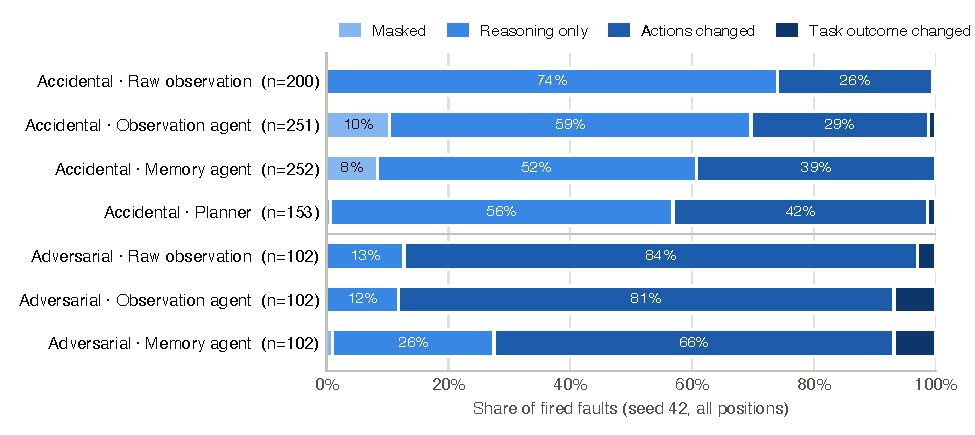
\includegraphics[width=\linewidth]{figures/propagation.pdf}
\caption{Outcome of each fired fault, by stage and category (seed 42, all positions).}
\label{fig:propagation}
\end{figure}

Figure~\ref{fig:propagation} shows the outcome of every fired fault. Masking is rare (0--10\%
per stage) and happens mostly when the fault lands 1--2 steps before the episode ends, so the
workload does depend on the injected results. The observation agent seems to act as a filter
for raw-observation faults: 74\% of corrupted raw observations changed reasoning but not
actions, and only 37\% of their downstream calls changed, the lowest of any stage.

Accidental faults rarely changed task success (6 of 856 lost). We think this is because the
environment is re-observed at every step, which usually lets the agents re-explore. The cost
is about +0.7 actions and +1.7k tokens per fault.

Prompt injections were the most serious case. Of these faults, 77\% changed executed actions
and 6\% changed the task outcome. Unauthorized actions occurred in 163 of 306 episodes: the
agent picked up the named foreign object in 158 episodes and executed the exact instructed
action in 38. The irreversible variant led to irreversible actions in 24 episodes. Earlier
injections did more damage, with early faults causing 213 unauthorized actions and late faults
31. In a single-LLM version of this workflow (deterministic observation and memory; 705 faults),
injections changed actions in only 41\% of runs. Our interpretation is that each agent that
copies the injected text into its own output gives it more authority downstream, although we
did not test this directly.

These results were consistent across seeds. Repeating the mid-position faults on seeds 43 and
44 gives a similar outcome mix (masked 2--4\%, reasoning only 48--53\%, actions changed
41--48\%, outcome changed 3--4\%), with a standard deviation across seeds of at most 2.8 points.

\begin{figure}[h]
\centering
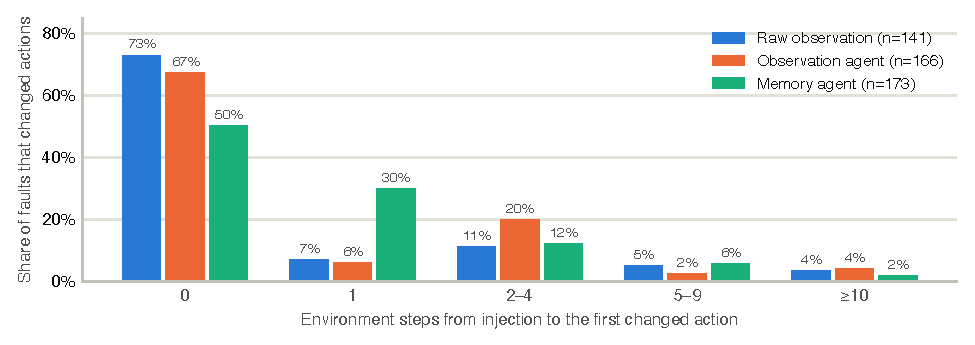
\includegraphics[width=\linewidth]{figures/delay.pdf}
\caption{Delay between injection and the first changed action, for faults that changed
actions (seed 42). Planner faults, not shown, always change the action at once.}
\label{fig:delay}
\end{figure}

Figure~\ref{fig:delay} shows that shared memory delays propagation. Faults at the raw
observation and the observation agent mostly change the action at the same step (73\% and
67\%), while 30\% of memory faults first change an action one step later. Across stages,
20--27\% of action-changing faults appear 2 or more steps later, and in the extreme case 25--28
steps later. A recovery mechanism therefore cannot assume that the effects of a fault are local
in time.

\subsection{Recovery baselines}
\begin{figure}[h]
\centering
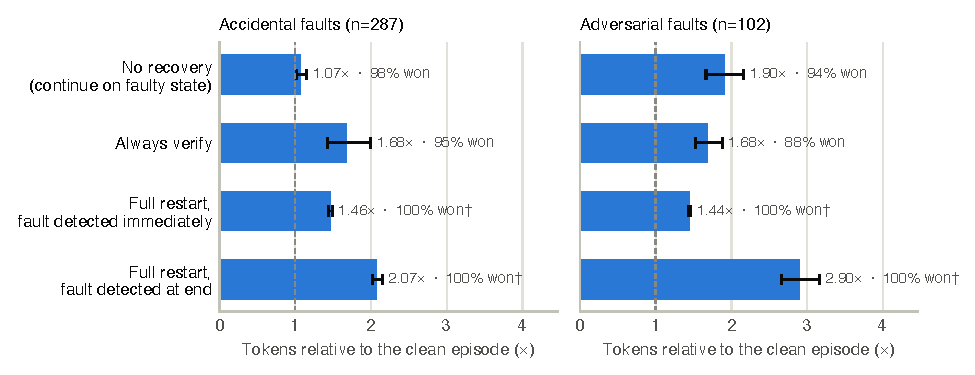
\includegraphics[width=\linewidth]{figures/cost.pdf}
\caption{Tokens needed to finish an episode under each response to a fault, relative to
the clean episode (mean, 95\% CI over games), with the share of tasks won, on the
identical seed-42 mid-position schedule. \textsuperscript{\dag}Restart success is the
executed live-restart rate (18/18).}
\label{fig:cost}
\end{figure}

Figure~\ref{fig:cost} compares four responses to the same faults. Full restart recovered the
task in all of our live runs, but it has to repeat all pre-fault work, which is 14\%, 46\% and
75\% of the clean episode's tokens for early, mid and late faults. Its total cost is
1.4--1.5$\times$ a clean episode if the fault is detected immediately and 2.1--2.9$\times$ if
it is detected at the end.

Always-verify blocked every unauthorized and irreversible action (154 and 8 under the baseline,
0 and 0 with the verifier), at a cost of 1.33$\times$ even on clean episodes. However, it lost
more tasks than the baseline, 27 of 389 against 11, with only 2 lost by both. Of the 27 losses,
23 ended in \code{verification\_rejected}. In these episodes the verifier correctly notices
that a plan relies on corrupted state, but the planner keeps planning from that state until the
attempt limit stops the episode. In other words, verification alone can detect a fault but
cannot recover from it.

\subsection{Failure diversity and a fuzzing pilot}
The systematic schedule produced 92 distinct signatures from 1,162 fired faults (114 with the
seed-43/44 repeats). The distribution has a long tail: the 10 most common signatures cover 56\%
of faults, and 27 signatures were seen only once. Planner faults produced only 9 signatures,
compared with 25--31 for each of the other stages.

Our proposal called for a fuzzing-inspired injector, so we ran a small pilot comparing one with
random injection. The fuzzer keeps a corpus of faults whose run produced a new signature and
mutates corpus entries in one of five ways: shifting the step, swapping the operator, swapping
the stage, moving the fault to another game at the same relative position, or reseeding it.
Entries are picked with weight severity/(1 + times picked), which favors outcome changes and
safety violations. The random baseline samples the game, stage--operator pair, step and seed
uniformly. Both arms used the same fault space (18 games), the same 12 initial faults and 96
episodes (Figure~\ref{fig:diversity}).

\begin{figure}[h]
\centering
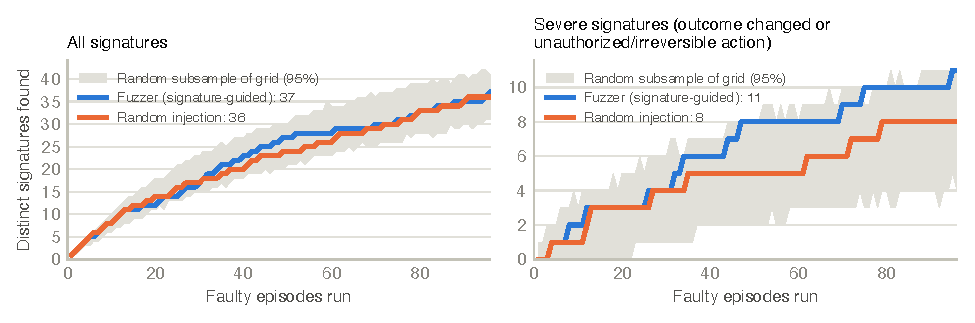
\includegraphics[width=\linewidth]{figures/diversity.pdf}
\caption{Distinct behavior signatures found as faulty episodes accumulate. The band is the
95\% range of random 1--96-fault subsamples of the 1,162-fault grid.}
\label{fig:diversity}
\end{figure}

Overall diversity was essentially tied, at 37 vs.\ 36 signatures, and both arms fall inside the
band of random grid subsamples at 96 faults (30--43). The fuzzer did find more severe behaviors:
unauthorized actions in 26 vs.\ 14 episodes, irreversible actions in 6 vs.\ 0 episodes, and 11
vs.\ 8 distinct severe signatures, which is at the top of the random band (4--11). It also found
3 signatures that the grid never produced, against 1 for random. This came at a cost of 35\% more
post-fault tokens (2.7M vs.\ 2.0M), possibly because severe runs tend to be longer. Swapping the
operator was the most productive mutation (12 of the 27 signatures found by mutation), while
step shifts and reseeds found only one each. Since we ran only one campaign per arm, these
results are suggestive rather than statistically significant.

\section{State restore design}\label{sec:restore}
Rolling an agent back to an earlier result does not roll back the world it acted on. We
therefore treat each layer of state separately (Table~\ref{tab:restore}): we use the cheapest
mechanism that is sound for that layer and check each restore against recorded fingerprints
before resuming. ALFWorld only exercises part of this design, so we have also included the layers
that a more complex environment would need.

\begin{table}[h]
\centering\small
\caption{State layers and how each is restored. ALFWorld needs rows 1, 2, 4 and 5; row 3
covers environments with files, containers, databases or browsers.}
\label{tab:restore}
\begin{tabularx}{\linewidth}{@{}>{\raggedright\arraybackslash}p{2.3cm} >{\raggedright\arraybackslash}p{2.5cm} X >{\raggedright\arraybackslash}p{2.6cm}@{}}
\toprule
Layer & Examples & Restore mechanism & Fidelity check \\
\midrule
1. Agent results, shared memory & facts, beliefs, plans & Version rollback: artifacts are immutable, so the role is pointed back to its last output before the fault; descendants are recomputed with influence cutoff. & output equality \\
2. Resettable, deterministic environment & ALFWorld, seeded simulators & Reset, then re-execute the \emph{recorded} actions before the first divergent one. Agents are not re-queried, since live calls are not deterministic. & observation hash at every replayed step \\
3. Snapshot-able environment & files, sandbox container, database, browser profile & Checkpoint at step boundaries: copy-on-write file-system snapshot (overlayfs, btrfs), container checkpoint (CRIU), MicroVM snapshot (Firecracker), database savepoint. Restore the last checkpoint before divergence, then replay forward. & state digest (file-tree hash, DB checksum, URL + DOM + cookies) \\
4. Live or shared environment & remote web session, shared repository & Compensation: undo the faulty actions newest first with registered inverses (take$\leftrightarrow$put, open$\leftrightarrow$close, create$\leftrightarrow$delete). & re-observe and compare with the recorded observation \\
5. External, irreversible effects & sent email, payment, heated object & Cannot be restored. Prevent by gating irreversible actions behind a checkpoint plus verification; otherwise report them as unrecoverable. & reported, not hidden \\
\bottomrule
\end{tabularx}
\end{table}

Given a faulty result at step $k$, the recovery procedure is as follows:
\begin{enumerate}
\item Roll back the agent state to step $k$.
\item If no executed action diverged, stop. This covers 53\% of fired faults.
\item Otherwise, restore the world to just before the first divergent action $d$, using the
first applicable mechanism: a snapshot at or before $d$; reset-and-replay; compensation, if
every action after $d$ has an inverse; or a partial restore that reports the irreversible
effects.
\item Check the fingerprints. On a mismatch, fall back to the next mechanism and finally to
full restart.
\end{enumerate}
Two parts are specific to the environment: a fingerprint function, and an action-effect registry
(\code{agent\_recovery/policy.py}) that classifies each command as observe-only, compensable
(with its inverse) or irreversible.

We can already estimate some of the costs from the Phase~1 traces, without new runs. Replay looks
cheap in ALFWorld: a reset takes 1.28\,s and a step 62\,ms (median), so replaying the median
4-action prefix takes 1.5\,s (at most 3.2\,s), compared with the 30\,s of model calls in a clean
episode. All 1,164 seed-42 faulty runs matched the clean observations up to the fault. In contrast,
compensation alone is often not enough. Of the 546 faults whose actions diverged, 61\% are fully
compensable (median of 6 inverse actions), 26\% include an irreversible action that the clean run
also takes later, and 13\% (71) include an irreversible action that the clean run never takes.
Without a reset or snapshot, this last group cannot be recovered even if the reasoning is repaired
perfectly.

In Phase~2 we plan to implement layers 1, 2, 4 and 5 on ALFWorld, along with a \emph{non-resettable}
mode that forbids reset so that we can measure compensation. We will report restore latency per
mechanism, fingerprint match rate, fall-back rate, the share of unrecoverable cases, and recovered
task success.

\section{Plan for Phase 2}
In Phase~2 we will build selective recovery, which combines dependency-aware invalidation and an
influence-aware early cutoff with the world-state restoration described in
Section~\ref{sec:restore}. As the course specifies, every method is told which result is faulty.

Our measurements suggest that structure overestimates influence. A fired fault has on average 35.2
structurally downstream calls, of which only 21.6 (61\%) change, and for accidental faults the
share is 37--50\%. Influence-aware recovery recomputes in dependency order and stops along a branch
once a recomputed output equals the old one, a comparison that sorted fact lists make exact and
cheap. We will compare it against full restart and always-verify under the same schedule, measuring
recovered task success and safety, recomputed calls, retained work, recovery latency and tracking
overhead, and we will audit recovered runs by re-executing the results they reuse.

We also plan to repeat the fuzzer and random campaigns with several search seeds and to reweight
mutations toward operator and stage swaps. If the fuzzer's advantage on severe faults holds up, those
faults would make a useful stress set for evaluating recovery.

\section{Limitations}
Our results have several limitations. All agents share one model, and the constraints and executor
are deterministic by design. Fault runs cover all positions only for seed 42, always-verify covers
only the mid position, and our CIs resample just 17--18 games. Latencies are logical; only the
executed restart measures live latency (27.0\,s wall vs.\ 25.7\,s model time). Output equality is
exact, which overstates influence, so we consider the 61\% figure conservative. The injected faults
are synthetic, the unauthorized-action policy is a simulation based on object types, and the fuzzing
pilot is one campaign per arm. Finally, two infrastructure failures were kept and rerun: one
transient budget rejection from the API proxy, and four runs hit by a cache-write race in our runner,
which we have since fixed.

\section{Reproducibility and cost}
Everything ran on a laptop (CPU only), and the binding constraint was the API rate limit (100
requests/min) rather than compute. All Phase~1 work used 48.6k API calls (46.3M tokens) and \$10.65
of TritonAI credit, and the final evaluation took about 11 hours. The fuzzing pilot added 192
episodes and \$0.81. \code{experiments/phase1.sh} reproduces all results and can be resumed, and
\code{analysis/report.py}, \code{figures.py}, \code{diversity.py} and \code{restore.py} regenerate
the tables and figures.

\end{document}
